\documentclass[tikz,border=5]{standalone}
\usepackage{amsmath,amssymb,graphicx,multirow,mathabx,mathtools,shuffle}
\usepackage{tikz}
\usepackage{tikz-qtree}
\usetikzlibrary{positioning}
\usetikzlibrary{fit,calc}

\begin{document}

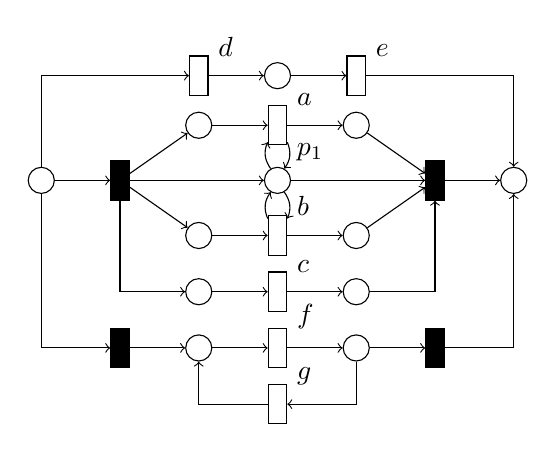
\begin{tikzpicture}
		[place/.style={draw, circle}, 
		transition/.style={draw, minimum height=0.5cm},
		silent transition/.style={transition, fill},
		treeNode/.style={draw, dashed}]
		
		\node (source) [place] {};
		
		%interleaved
		\def\firstone{7mm}
		\def\secondone{7mm};
		\def\milestoneplace{5mm};
		\def\dist{3.3mm};
		\node (int1) [silent transition, right of=source] {};
		
		\node (int12) [place, right of=int1, yshift=\secondone] {};
		\node (int112) [place, right of=int1, yshift=-\secondone] {};
		\node (a) [transition, right of=int12, label=above right:$a$] {};
		\node (int16) [place, right of=a] {};
		
		\node (b) [transition, right of=int112, label=above right:$b$] {};
		\node (int23) [place, right of=b] {};
		\node (milestone) [place, label=above right:$p_1$] at ($(a)!0.5!(b)$) {};
		
		\node (c) [transition, below=2mm of b, label=above right:$c$] {};		
		\node (int4) [place, left of=c] {};
		\node (int6) [place, right of=c] {};
		
		\node (int9) [silent transition, right of=int16, yshift=-\firstone] {};
		
		\draw [->] (source) to (int1);
		\draw [->] (int1) |- (int4);
		\draw [->] (int4) to (c);
		\draw [->] (c) to (int6);
		\draw [->] (int6) -| (int9);
		\draw [->] (int1) to (int12);
		\draw [->] (int12) to (a);
		\draw [->] (a) to (int16);
		\draw [->] (int16) to (int9);
		\draw [->] (int112) to (b);
		\draw [->] (int1) to (int112);
		\draw [->] (int1) to (milestone);
		\draw [->, bend left] (milestone) to (a);
		\draw [->, bend left] (milestone) to (b);
		\draw [->, bend left] (a) to (milestone);
		\draw [->, bend left] (b) to (milestone);
		\draw [->] (b) to (int23);
		\draw [->] (int23) to (int9);
		\draw [->] (milestone) to (int9);
		
		%sequence
		\node (seq2) [place, above=2mm of a] {};
		\node (seq1) [transition, left of=seq2, label=above right:$d$] {};
		\node (seq3) [transition, right of=seq2, label=above right:$e$] {};
		
		\draw [->] (source) |- (seq1);
		\draw [->] (seq1) to (seq2);
		\draw [->] (seq2) to (seq3);
		
		%loop
		\node (loop3) [transition, below=2mm of c, label=above right:$f$] {};
		\node (loop2) [place, left of=loop3] {};
		\node (loop1) [silent transition, left of=loop2] {};		
		\node (loop4) [place, right of=loop3] {};
		\node (loop5) [transition, below=2mm of loop3, label=above right:$g$] {};
		\node (loop6) [silent transition, right of=loop4] {};

		\draw [->] (source) |- (loop1);		
		\draw [->] (loop1) to (loop2);
		\draw [->] (loop2) to (loop3);
		\draw [->] (loop3) to (loop4);
		\draw [->] (loop4) |- (loop5);
		\draw [->] (loop5) -| (loop2);
		\draw [->] (loop4) to (loop6);
		
		%sink
		\node (sink) [place, right of=int9] {};
		\draw [->] (loop6) -| (sink);
		\draw [->] (seq3) -| (sink);
		\draw [->] (int9) to (sink);
		
	\end{tikzpicture}

\end{document}